% Options for packages loaded elsewhere
\PassOptionsToPackage{unicode}{hyperref}
\PassOptionsToPackage{hyphens}{url}
%
\documentclass[
]{article}
\usepackage{amsmath,amssymb}
\usepackage{iftex}
\ifPDFTeX
  \usepackage[T1]{fontenc}
  \usepackage[utf8]{inputenc}
  \usepackage{textcomp} % provide euro and other symbols
\else % if luatex or xetex
  \usepackage{unicode-math} % this also loads fontspec
  \defaultfontfeatures{Scale=MatchLowercase}
  \defaultfontfeatures[\rmfamily]{Ligatures=TeX,Scale=1}
\fi
\usepackage{lmodern}
\ifPDFTeX\else
  % xetex/luatex font selection
\fi
% Use upquote if available, for straight quotes in verbatim environments
\IfFileExists{upquote.sty}{\usepackage{upquote}}{}
\IfFileExists{microtype.sty}{% use microtype if available
  \usepackage[]{microtype}
  \UseMicrotypeSet[protrusion]{basicmath} % disable protrusion for tt fonts
}{}
\makeatletter
\@ifundefined{KOMAClassName}{% if non-KOMA class
  \IfFileExists{parskip.sty}{%
    \usepackage{parskip}
  }{% else
    \setlength{\parindent}{0pt}
    \setlength{\parskip}{6pt plus 2pt minus 1pt}}
}{% if KOMA class
  \KOMAoptions{parskip=half}}
\makeatother
\usepackage{xcolor}
\usepackage[margin=1in]{geometry}
\usepackage{color}
\usepackage{fancyvrb}
\newcommand{\VerbBar}{|}
\newcommand{\VERB}{\Verb[commandchars=\\\{\}]}
\DefineVerbatimEnvironment{Highlighting}{Verbatim}{commandchars=\\\{\}}
% Add ',fontsize=\small' for more characters per line
\usepackage{framed}
\definecolor{shadecolor}{RGB}{248,248,248}
\newenvironment{Shaded}{\begin{snugshade}}{\end{snugshade}}
\newcommand{\AlertTok}[1]{\textcolor[rgb]{0.94,0.16,0.16}{#1}}
\newcommand{\AnnotationTok}[1]{\textcolor[rgb]{0.56,0.35,0.01}{\textbf{\textit{#1}}}}
\newcommand{\AttributeTok}[1]{\textcolor[rgb]{0.13,0.29,0.53}{#1}}
\newcommand{\BaseNTok}[1]{\textcolor[rgb]{0.00,0.00,0.81}{#1}}
\newcommand{\BuiltInTok}[1]{#1}
\newcommand{\CharTok}[1]{\textcolor[rgb]{0.31,0.60,0.02}{#1}}
\newcommand{\CommentTok}[1]{\textcolor[rgb]{0.56,0.35,0.01}{\textit{#1}}}
\newcommand{\CommentVarTok}[1]{\textcolor[rgb]{0.56,0.35,0.01}{\textbf{\textit{#1}}}}
\newcommand{\ConstantTok}[1]{\textcolor[rgb]{0.56,0.35,0.01}{#1}}
\newcommand{\ControlFlowTok}[1]{\textcolor[rgb]{0.13,0.29,0.53}{\textbf{#1}}}
\newcommand{\DataTypeTok}[1]{\textcolor[rgb]{0.13,0.29,0.53}{#1}}
\newcommand{\DecValTok}[1]{\textcolor[rgb]{0.00,0.00,0.81}{#1}}
\newcommand{\DocumentationTok}[1]{\textcolor[rgb]{0.56,0.35,0.01}{\textbf{\textit{#1}}}}
\newcommand{\ErrorTok}[1]{\textcolor[rgb]{0.64,0.00,0.00}{\textbf{#1}}}
\newcommand{\ExtensionTok}[1]{#1}
\newcommand{\FloatTok}[1]{\textcolor[rgb]{0.00,0.00,0.81}{#1}}
\newcommand{\FunctionTok}[1]{\textcolor[rgb]{0.13,0.29,0.53}{\textbf{#1}}}
\newcommand{\ImportTok}[1]{#1}
\newcommand{\InformationTok}[1]{\textcolor[rgb]{0.56,0.35,0.01}{\textbf{\textit{#1}}}}
\newcommand{\KeywordTok}[1]{\textcolor[rgb]{0.13,0.29,0.53}{\textbf{#1}}}
\newcommand{\NormalTok}[1]{#1}
\newcommand{\OperatorTok}[1]{\textcolor[rgb]{0.81,0.36,0.00}{\textbf{#1}}}
\newcommand{\OtherTok}[1]{\textcolor[rgb]{0.56,0.35,0.01}{#1}}
\newcommand{\PreprocessorTok}[1]{\textcolor[rgb]{0.56,0.35,0.01}{\textit{#1}}}
\newcommand{\RegionMarkerTok}[1]{#1}
\newcommand{\SpecialCharTok}[1]{\textcolor[rgb]{0.81,0.36,0.00}{\textbf{#1}}}
\newcommand{\SpecialStringTok}[1]{\textcolor[rgb]{0.31,0.60,0.02}{#1}}
\newcommand{\StringTok}[1]{\textcolor[rgb]{0.31,0.60,0.02}{#1}}
\newcommand{\VariableTok}[1]{\textcolor[rgb]{0.00,0.00,0.00}{#1}}
\newcommand{\VerbatimStringTok}[1]{\textcolor[rgb]{0.31,0.60,0.02}{#1}}
\newcommand{\WarningTok}[1]{\textcolor[rgb]{0.56,0.35,0.01}{\textbf{\textit{#1}}}}
\usepackage{longtable,booktabs,array}
\usepackage{calc} % for calculating minipage widths
% Correct order of tables after \paragraph or \subparagraph
\usepackage{etoolbox}
\makeatletter
\patchcmd\longtable{\par}{\if@noskipsec\mbox{}\fi\par}{}{}
\makeatother
% Allow footnotes in longtable head/foot
\IfFileExists{footnotehyper.sty}{\usepackage{footnotehyper}}{\usepackage{footnote}}
\makesavenoteenv{longtable}
\usepackage{graphicx}
\makeatletter
\def\maxwidth{\ifdim\Gin@nat@width>\linewidth\linewidth\else\Gin@nat@width\fi}
\def\maxheight{\ifdim\Gin@nat@height>\textheight\textheight\else\Gin@nat@height\fi}
\makeatother
% Scale images if necessary, so that they will not overflow the page
% margins by default, and it is still possible to overwrite the defaults
% using explicit options in \includegraphics[width, height, ...]{}
\setkeys{Gin}{width=\maxwidth,height=\maxheight,keepaspectratio}
% Set default figure placement to htbp
\makeatletter
\def\fps@figure{htbp}
\makeatother
\setlength{\emergencystretch}{3em} % prevent overfull lines
\providecommand{\tightlist}{%
  \setlength{\itemsep}{0pt}\setlength{\parskip}{0pt}}
\setcounter{secnumdepth}{-\maxdimen} % remove section numbering
\ifLuaTeX
  \usepackage{selnolig}  % disable illegal ligatures
\fi
\IfFileExists{bookmark.sty}{\usepackage{bookmark}}{\usepackage{hyperref}}
\IfFileExists{xurl.sty}{\usepackage{xurl}}{} % add URL line breaks if available
\urlstyle{same}
\hypersetup{
  pdftitle={E-commerceDB},
  pdfauthor={Group-8},
  hidelinks,
  pdfcreator={LaTeX via pandoc}}

\title{E-commerceDB}
\author{Group-8}
\date{2024-02-27}

\begin{document}
\maketitle

\hypertarget{load-necessary-libraries}{%
\section{Load necessary libraries}\label{load-necessary-libraries}}

\begin{Shaded}
\begin{Highlighting}[]
\FunctionTok{library}\NormalTok{(DBI)}
\FunctionTok{library}\NormalTok{(readr)}
\FunctionTok{library}\NormalTok{(RSQLite)}
\FunctionTok{library}\NormalTok{(dplyr)}
\end{Highlighting}
\end{Shaded}

\begin{verbatim}
## 
## Attaching package: 'dplyr'
\end{verbatim}

\begin{verbatim}
## The following objects are masked from 'package:stats':
## 
##     filter, lag
\end{verbatim}

\begin{verbatim}
## The following objects are masked from 'package:base':
## 
##     intersect, setdiff, setequal, union
\end{verbatim}

\begin{Shaded}
\begin{Highlighting}[]
\FunctionTok{library}\NormalTok{(stringr)}
\end{Highlighting}
\end{Shaded}

\begin{Shaded}
\begin{Highlighting}[]
\NormalTok{con }\OtherTok{\textless{}{-}} \FunctionTok{dbConnect}\NormalTok{(RSQLite}\SpecialCharTok{::}\FunctionTok{SQLite}\NormalTok{(), }\StringTok{"ecommerce.db"}\NormalTok{)}
\CommentTok{\# on.exit(dbDisconnect(con), add = TRUE)}

\NormalTok{sql\_file }\OtherTok{\textless{}{-}} \FunctionTok{readLines}\NormalTok{(}\StringTok{"dbScript.sql"}\NormalTok{)}

\ControlFlowTok{for}\NormalTok{ (sql\_command }\ControlFlowTok{in}\NormalTok{ sql\_file) \{}
  \ControlFlowTok{if}\NormalTok{ (sql\_command}\SpecialCharTok{!=}\StringTok{""}\NormalTok{)\{}
    \FunctionTok{print}\NormalTok{(sql\_command)}
    \FunctionTok{dbExecute}\NormalTok{(con,sql\_command)}
    \FunctionTok{print}\NormalTok{(}\StringTok{"{-}{-}{-}{-}{-}{-}{-}{-}{-}{-}{-}{-}{-}DONE{-}{-}{-}{-}{-}{-}{-}{-}{-}"}\NormalTok{)}
\NormalTok{  \}}
\NormalTok{\}}
\end{Highlighting}
\end{Shaded}

\begin{verbatim}
## [1] "CREATE TABLE IF NOT EXISTS 'Category'( 'Category_ID' VARCHAR(250) PRIMARY KEY, 'Category_Name' VARCHAR(250) NOT NULL );"
## [1] "-------------DONE---------"
## [1] "CREATE TABLE IF NOT EXISTS 'Suppliers'( 'Supplier_ID' VARCHAR(250) PRIMARY KEY, 'Supplier_Name' VARCHAR(250) NOT NULL, 'Supplier_Building_Name' VARCHAR(250), 'Supplier_Street_Name' VARCHAR(250) NOT NULL, 'Supplier_Zip' VARCHAR(250) NOT NULL, 'Supplier_Email' VARCHAR(250) NOT NULL, 'Supplier_Status' VARCHAR(250) NOT NULL );"
## [1] "-------------DONE---------"
## [1] "CREATE TABLE IF NOT EXISTS 'Discounts'( 'Discount_Code' VARCHAR(50) PRIMARY KEY, 'Discount_Amount' FLOAT(10,2) NOT NULL, 'Discount_Status' BOOLEAN NOT NULL, 'Category_ID' VARCHAR(250) NOT NULL, 'Product_ID' VARCHAR(250) NOT NULL, FOREIGN KEY ('Category_ID') REFERENCES Category('Category_ID'), FOREIGN KEY ('Product_ID') REFERENCES Products('Product_ID') );"
## [1] "-------------DONE---------"
## [1] "CREATE TABLE IF NOT EXISTS 'Products' ( 'Product_ID' VARCHAR(250) PRIMARY KEY, 'Product_Name' VARCHAR(250) NOT NULL, 'Product_Availability' VARCHAR(25) , 'Product_Price' FLOAT(10,2) NOT NULL, 'Category_ID' VARCHAR(250) NOT NULL,'Supplier_ID' VARCHAR(250) NOT NULL, 'Discount_Code' VARCHAR(250),FOREIGN KEY ('Category_ID') REFERENCES Category(Category_ID), FOREIGN KEY ('Supplier_ID') REFERENCES Suppliers(Supplier_ID), FOREIGN KEY ('Discount_Code') REFERENCES Discounts('Discount_Code')); "
## [1] "-------------DONE---------"
## [1] "CREATE TABLE IF NOT EXISTS 'Customers' ( 'Cust_ID' VARCHAR(250) PRIMARY KEY, 'Cust_Name' VARCHAR(250) NOT NULL, 'Cust_Building_Name' VARCHAR(250) , 'Cust_Street_Name' VARCHAR(250) NOT NULL, 'Cust_Zip' VARCHAR(25) NOT NULL, 'Cust_Email' VARCHAR(250) NOT NULL, 'Cust_Phone_Number' INT NOT NULL, 'Cust_Country_Code' VARCHAR(250) );"
## [1] "-------------DONE---------"
## [1] "CREATE TABLE IF NOT EXISTS 'Reviews' ( 'Review_ID' VARCHAR(50) PRIMARY KEY,'Review_Timestamp' DATETIME NOT NULL, 'Product_Rating' INT NOT NULL, 'Review_Text' TEXT, 'Review_Likes' INT, 'Product_ID' VARCHAR(250) NOT NULL, FOREIGN KEY ('Product_ID') REFERENCES Products('Product_ID') );"
## [1] "-------------DONE---------"
## [1] "CREATE TABLE IF NOT EXISTS 'Order_Items'( 'Quantity' INT NOT NULL, 'Sum_Price' INT NOT NULL, 'Order_ID' VARCHAR(250) NOT NULL,'Product_ID' VARCHAR(250) NOT NULL, PRIMARY KEY ('Order_ID','Product_ID'), FOREIGN KEY ('Order_ID') REFERENCES Orders('Order_ID'), FOREIGN KEY ('Product_ID') REFERENCES Products('Product_ID'));"
## [1] "-------------DONE---------"
## [1] "CREATE TABLE IF NOT EXISTS 'Order_Details' ( 'Order_ID'  VARCHAR(250) PRIMARY KEY, 'Order_Date' DATETIME NOT NULL, 'Shipping_Building_Name' VARCHAR(250), 'Shipping_Street_Name' VARCHAR(250) NOT NULL, 'Shipping_Zip_Code' VARCHAR(250) NOT NULL, 'Order_Total' FLOAT(10,2) NOT NULL, 'Order_Status' VARCHAR(50) NOT NULL, 'Payment_Type' VARCHAR(50) NOT NULL, 'Payment_Status' VARCHAR(50) NOT NULL, 'Billing_Building_Name' VARCHAR(250), 'Billing_Street_Name' VARCHAR(250) NOT NULL, 'Billing_Zip_Code' VARCHAR(50) NOT NULL, 'Cust_ID' VARCHAR(250) NOT NULL, 'Discount_Code' VARCHAR(250) NOT NULL, FOREIGN KEY ('Cust_ID') REFERENCES Customers('Cust_ID'));"
## [1] "-------------DONE---------"
## [1] "CREATE TABLE IF NOT EXISTS 'Products' ( 'Product_ID' VARCHAR(250) PRIMARY KEY, 'Product_Name' VARCHAR(250) NOT NULL, 'Product_Availability' VARCHAR(25) , 'Product_Price' FLOAT(10,2) NOT NULL, 'Category_ID' VARCHAR(250) NOT NULL,'Supplier_ID' VARCHAR(250) NOT NULL,FOREIGN KEY ('Category_ID') REFERENCES Category(Category_ID), FOREIGN KEY ('Supplier_ID') REFERENCES Suppliers(Supplier_ID)); "
## [1] "-------------DONE---------"
## [1] "CREATE TABLE IF NOT EXISTS 'Customers' ( 'Cust_ID' VARCHAR(250) PRIMARY KEY, 'Cust_Name' VARCHAR(250) NOT NULL, 'Cust_Building_Name' VARCHAR(250) , 'Cust_Street_Name' VARCHAR(250) NOT NULL, 'Cust_Zip' VARCHAR(25) NOT NULL, 'Cust_Email' VARCHAR(250) NOT NULL, 'Cust_Phone_Number' INT NOT NULL, 'Cust_Country_Code' VARCHAR(250) );"
## [1] "-------------DONE---------"
## [1] "CREATE TABLE IF NOT EXISTS 'Reviews' ( 'Review_ID' VARCHAR(50) PRIMARY KEY,'Review_Timestamp' DATETIME NOT NULL, 'Product_Rating' INT NOT NULL, 'Review_Text' TEXT, 'Review_Likes' INT, 'Product_ID' VARCHAR(250) NOT NULL, FOREIGN KEY ('Product_ID') REFERENCES Products('Product_ID') );"
## [1] "-------------DONE---------"
## [1] "CREATE TABLE IF NOT EXISTS 'Discounts'( 'Discount_Code' VARCHAR(50) PRIMARY KEY, 'Discount_Amount' FLOAT(10,2) NOT NULL, 'Discount_Status' BOOLEAN NOT NULL, 'Category_ID' VARCHAR(250) NOT NULL, 'Product_ID' VARCHAR(250) NOT NULL, FOREIGN KEY ('Category_ID') REFERENCES Category('Category_ID'), FOREIGN KEY ('Product_ID') REFERENCES Products('Product_ID') );"
## [1] "-------------DONE---------"
## [1] "CREATE TABLE IF NOT EXISTS 'Order_Items'( 'Quantity' INT NOT NULL, 'Sum_Price' INT NOT NULL, 'Order_ID' VARCHAR(250) NOT NULL,'Product_ID' VARCHAR(250) NOT NULL, PRIMARY KEY ('Order_ID','Product_ID'), FOREIGN KEY ('Order_ID') REFERENCES Orders('Order_ID'), FOREIGN KEY ('Product_ID') REFERENCES Products('Product_ID'));"
## [1] "-------------DONE---------"
## [1] "CREATE TABLE IF NOT EXISTS 'Order_Details' ( 'Order_ID'  VARCHAR(250) PRIMARY KEY, 'Order_Date' DATETIME NOT NULL, 'Shipping_Building_Name' VARCHAR(250), 'Shipping_Street_Name' VARCHAR(250) NOT NULL, 'Shipping_Zip_Code' VARCHAR(250) NOT NULL, 'Discount' VARCHAR(250) NOT NULL, 'Order_Total' FLOAT(10,2) NOT NULL, 'Order_Status' VARCHAR(50) NOT NULL, 'Payment_Type' VARCHAR(50) NOT NULL, 'Payment_Status' VARCHAR(50) NOT NULL, 'Billing_Building_Name' VARCHAR(250), 'Billing_Street_Name' VARCHAR(250) NOT NULL, 'Billing_Zip' VARCHAR(50) NOT NULL, 'Cust_ID' VARCHAR(250) NOT NULL, 'Discount_Code' VARCHAR(250) NOT NULL, FOREIGN KEY ('Cust_ID') REFERENCES Customers('Cust_ID'), FOREIGN KEY ('Discount_Code') REFERENCES DISCOUNTS('Discount_Code') );"
## [1] "-------------DONE---------"
\end{verbatim}

\begin{Shaded}
\begin{Highlighting}[]
\CommentTok{\# Disconnect}
\FunctionTok{dbDisconnect}\NormalTok{(con)}
\end{Highlighting}
\end{Shaded}

\begin{Shaded}
\begin{Highlighting}[]
\NormalTok{con }\OtherTok{\textless{}{-}} \FunctionTok{dbConnect}\NormalTok{(RSQLite}\SpecialCharTok{::}\FunctionTok{SQLite}\NormalTok{(), }\StringTok{"ecommerce.db"}\NormalTok{)}

\CommentTok{\# con \textless{}{-} dbConnect(RSQLite::SQLite(), "ecommerce.db")}


\NormalTok{Customers }\OtherTok{\textless{}{-}} \FunctionTok{read\_csv}\NormalTok{(}\StringTok{"Files/Customers.csv"}\NormalTok{)}
\end{Highlighting}
\end{Shaded}

\begin{verbatim}
## Rows: 150 Columns: 10
## -- Column specification --------------------------------------------------------
## Delimiter: ","
## chr (7): Cust_ID, Cust_First_Name, Cust_Last_Name, Cust_Building_Name, Cust_...
## dbl (3): Cust_Building_Number, Cust_Phone_Number, Phone_Country_Code
## 
## i Use `spec()` to retrieve the full column specification for this data.
## i Specify the column types or set `show_col_types = FALSE` to quiet this message.
\end{verbatim}

\begin{Shaded}
\begin{Highlighting}[]
\NormalTok{Products }\OtherTok{\textless{}{-}} \FunctionTok{read\_csv}\NormalTok{(}\StringTok{"Files/Products.csv"}\NormalTok{)}
\end{Highlighting}
\end{Shaded}

\begin{verbatim}
## Rows: 150 Columns: 4
## -- Column specification --------------------------------------------------------
## Delimiter: ","
## chr (3): Product_ID, Product_Name, Product_Availability
## dbl (1): Product_Price
## 
## i Use `spec()` to retrieve the full column specification for this data.
## i Specify the column types or set `show_col_types = FALSE` to quiet this message.
\end{verbatim}

\begin{Shaded}
\begin{Highlighting}[]
\NormalTok{Order\_details }\OtherTok{\textless{}{-}} \FunctionTok{read\_csv}\NormalTok{(}\StringTok{"Files/Order\_Details.csv"}\NormalTok{,}
    \AttributeTok{skip =} \DecValTok{1}\NormalTok{)}
\end{Highlighting}
\end{Shaded}

\begin{verbatim}
## Rows: 150 Columns: 13
## -- Column specification --------------------------------------------------------
## Delimiter: ","
## chr  (10): Order_ID, Shipping_Building_Name, Shipping_Street_Name, Shipping_...
## dbl   (2): Shipping_Building_Number, Billing_Building_Number
## dttm  (1): Order_Date
## 
## i Use `spec()` to retrieve the full column specification for this data.
## i Specify the column types or set `show_col_types = FALSE` to quiet this message.
\end{verbatim}

\begin{Shaded}
\begin{Highlighting}[]
\NormalTok{Reviews }\OtherTok{\textless{}{-}} \FunctionTok{read\_csv}\NormalTok{(}\StringTok{"Files/Reviews.csv"}\NormalTok{,}
    \AttributeTok{skip =} \DecValTok{1}\NormalTok{)}
\end{Highlighting}
\end{Shaded}

\begin{verbatim}
## Rows: 150 Columns: 5
## -- Column specification --------------------------------------------------------
## Delimiter: ","
## chr  (2): Review_ID, Review_Text
## dbl  (2): Product_Rating, Review_Likes
## dttm (1): Review_Timestamp
## 
## i Use `spec()` to retrieve the full column specification for this data.
## i Specify the column types or set `show_col_types = FALSE` to quiet this message.
\end{verbatim}

\begin{Shaded}
\begin{Highlighting}[]
\NormalTok{Suppliers }\OtherTok{\textless{}{-}} \FunctionTok{read\_csv}\NormalTok{(}\StringTok{"Files/Suppliers.csv"}\NormalTok{)}
\end{Highlighting}
\end{Shaded}

\begin{verbatim}
## Rows: 50 Columns: 8
## -- Column specification --------------------------------------------------------
## Delimiter: ","
## chr (6): Supplier_ID, Supplier_Name, Supplier_Building_Name, Supplier_Street...
## dbl (2): Supplier_Building_Number, Supplier_Zip_Code
## 
## i Use `spec()` to retrieve the full column specification for this data.
## i Specify the column types or set `show_col_types = FALSE` to quiet this message.
\end{verbatim}

\begin{Shaded}
\begin{Highlighting}[]
\NormalTok{Product\_Discounts }\OtherTok{\textless{}{-}} \FunctionTok{read\_csv}\NormalTok{(}\StringTok{"Files/Product\_Discounts.csv"}\NormalTok{)}
\end{Highlighting}
\end{Shaded}

\begin{verbatim}
## Rows: 50 Columns: 3
## -- Column specification --------------------------------------------------------
## Delimiter: ","
## chr (1): Discount_Code
## dbl (1): Discount_Amount
## lgl (1): Discount_Status
## 
## i Use `spec()` to retrieve the full column specification for this data.
## i Specify the column types or set `show_col_types = FALSE` to quiet this message.
\end{verbatim}

\begin{Shaded}
\begin{Highlighting}[]
\NormalTok{Product\_Category }\OtherTok{\textless{}{-}} \FunctionTok{read\_csv}\NormalTok{(}\StringTok{"Files/Product\_Category.csv"}\NormalTok{)}
\end{Highlighting}
\end{Shaded}

\begin{verbatim}
## Rows: 10 Columns: 2
## -- Column specification --------------------------------------------------------
## Delimiter: ","
## chr (2): Category_ID, Category_Name
## 
## i Use `spec()` to retrieve the full column specification for this data.
## i Specify the column types or set `show_col_types = FALSE` to quiet this message.
\end{verbatim}

\begin{Shaded}
\begin{Highlighting}[]
\NormalTok{Order\_Item }\OtherTok{\textless{}{-}} \FunctionTok{read\_csv}\NormalTok{(}\StringTok{"Files/Order\_Item.csv"}\NormalTok{, }
    \AttributeTok{skip =} \DecValTok{1}\NormalTok{)}
\end{Highlighting}
\end{Shaded}

\begin{verbatim}
## Rows: 200 Columns: 1
## -- Column specification --------------------------------------------------------
## Delimiter: ","
## dbl (1): Order_Item
## 
## i Use `spec()` to retrieve the full column specification for this data.
## i Specify the column types or set `show_col_types = FALSE` to quiet this message.
\end{verbatim}

\begin{Shaded}
\begin{Highlighting}[]
\CommentTok{\# To create empty column for the Products table }
\NormalTok{Products }\OtherTok{\textless{}{-}}\NormalTok{ Products }\SpecialCharTok{\%\textgreater{}\%}
  \FunctionTok{mutate}\NormalTok{(}\AttributeTok{Category\_ID =} \ConstantTok{NA}\NormalTok{)}

\CommentTok{\# To apply the foreign key into the table }
\CommentTok{\# Define a function to assign Category\_ID based on keywords in Product\_Name}
\NormalTok{assign\_category\_id }\OtherTok{\textless{}{-}} \ControlFlowTok{function}\NormalTok{(Product\_Name) \{}
  \ControlFlowTok{if}\NormalTok{ (}\FunctionTok{grepl}\NormalTok{(}\StringTok{"TV|Television"}\NormalTok{, Product\_Name, }\AttributeTok{ignore.case =} \ConstantTok{TRUE}\NormalTok{)) \{}
    \FunctionTok{return}\NormalTok{(}\StringTok{"CAT1"}\NormalTok{)}
\NormalTok{  \} }\ControlFlowTok{else} \ControlFlowTok{if}\NormalTok{ (}\FunctionTok{grepl}\NormalTok{(}\StringTok{"Laptop|Tablet|Computing|Book|Surface|Monitor"}\NormalTok{, Product\_Name, }\AttributeTok{ignore.case =} \ConstantTok{TRUE}\NormalTok{)) \{}
    \FunctionTok{return}\NormalTok{(}\StringTok{"CAT2"}\NormalTok{)}
\NormalTok{  \} }\ControlFlowTok{else} \ControlFlowTok{if}\NormalTok{ (}\FunctionTok{grepl}\NormalTok{(}\StringTok{"Phone|Galaxy|Mi|P Series|OnePlus"}\NormalTok{, Product\_Name, }\AttributeTok{ignore.case =} \ConstantTok{TRUE}\NormalTok{)) \{}
    \FunctionTok{return}\NormalTok{(}\StringTok{"CAT3"}\NormalTok{)}
\NormalTok{  \} }\ControlFlowTok{else} \ControlFlowTok{if}\NormalTok{ (}\FunctionTok{grepl}\NormalTok{(}\StringTok{"Refrigerator|Washing Machine|Home Appliance|Microwave|Vacuum|Dishwasher"}\NormalTok{, Product\_Name, }\AttributeTok{ignore.case =} \ConstantTok{TRUE}\NormalTok{))\{}
    \FunctionTok{return}\NormalTok{(}\StringTok{"CAT4"}\NormalTok{)}
\NormalTok{  \} }\ControlFlowTok{else} \ControlFlowTok{if}\NormalTok{ (}\FunctionTok{grepl}\NormalTok{(}\StringTok{"Headphones|Speakers|Sound System|Earbuds|Speaker|Technica|Soundbar"}\NormalTok{, Product\_Name, }\AttributeTok{ignore.case =} \ConstantTok{TRUE}\NormalTok{)) \{}
    \FunctionTok{return}\NormalTok{(}\StringTok{"CAT5"}\NormalTok{)}
\NormalTok{  \} }\ControlFlowTok{else} \ControlFlowTok{if}\NormalTok{ (}\FunctionTok{grepl}\NormalTok{(}\StringTok{"Camera|Photography|GoPro|Mirrorless|Nikon|Camcorder|Compact"}\NormalTok{, Product\_Name, }\AttributeTok{ignore.case =} \ConstantTok{TRUE}\NormalTok{)) \{}
    \FunctionTok{return}\NormalTok{(}\StringTok{"CAT6"}\NormalTok{)}
\NormalTok{  \} }\ControlFlowTok{else} \ControlFlowTok{if}\NormalTok{ (}\FunctionTok{grepl}\NormalTok{(}\StringTok{"Xbox|PS|Gaming|Switch"}\NormalTok{, Product\_Name, }\AttributeTok{ignore.case =} \ConstantTok{TRUE}\NormalTok{)) \{}
    \FunctionTok{return}\NormalTok{(}\StringTok{"CAT7"}\NormalTok{)}
\NormalTok{  \} }\ControlFlowTok{else} \ControlFlowTok{if}\NormalTok{ (}\FunctionTok{grepl}\NormalTok{(}\StringTok{"Smart Home|Echo|Smart Lock|Steam Deck|Hue Light"}\NormalTok{, Product\_Name, }\AttributeTok{ignore.case =} \ConstantTok{TRUE}\NormalTok{)) \{}
    \FunctionTok{return}\NormalTok{(}\StringTok{"CAT8"}\NormalTok{)}
\NormalTok{  \} }\ControlFlowTok{else} \ControlFlowTok{if}\NormalTok{ (}\FunctionTok{grepl}\NormalTok{(}\StringTok{"Watch|Wearable|Quest|Tracker|Gear|Band|Glasses"}\NormalTok{, Product\_Name, }\AttributeTok{ignore.case =} \ConstantTok{TRUE}\NormalTok{)) \{}
    \FunctionTok{return}\NormalTok{(}\StringTok{"CAT9"}\NormalTok{)}
\NormalTok{  \} }\ControlFlowTok{else} \ControlFlowTok{if}\NormalTok{ (}\FunctionTok{grepl}\NormalTok{(}\StringTok{"Keyboard|Mouse|Peripheral|Thermostat"}\NormalTok{, Product\_Name, }\AttributeTok{ignore.case =} \ConstantTok{TRUE}\NormalTok{)) \{}
    \FunctionTok{return}\NormalTok{(}\StringTok{"CAT10"}\NormalTok{)}
\NormalTok{  \} }\ControlFlowTok{else}\NormalTok{ \{}
    \FunctionTok{return}\NormalTok{(}\ConstantTok{NA}\NormalTok{) }\CommentTok{\# For products that do not match any category}
\NormalTok{  \}}
\NormalTok{\}}

\CommentTok{\# Apply the function to assign Category\_ID to each product}
\NormalTok{Products}\SpecialCharTok{$}\NormalTok{Category\_ID }\OtherTok{\textless{}{-}} \FunctionTok{sapply}\NormalTok{(Products}\SpecialCharTok{$}\NormalTok{Product\_Name, assign\_category\_id)}
\end{Highlighting}
\end{Shaded}

\begin{Shaded}
\begin{Highlighting}[]
\CommentTok{\# This is to add suppliers\_id in Products}
\FunctionTok{set.seed}\NormalTok{(}\DecValTok{123}\NormalTok{)}

\NormalTok{Products }\OtherTok{\textless{}{-}}\NormalTok{ Products }\SpecialCharTok{\%\textgreater{}\%}
  \FunctionTok{mutate}\NormalTok{(}\AttributeTok{Supplier\_ID =} \ConstantTok{NA}\NormalTok{)}

\CommentTok{\# Create a function to find matching supplier ID or assign randomly if no match is found}
\NormalTok{assign\_supplier\_id }\OtherTok{\textless{}{-}} \ControlFlowTok{function}\NormalTok{(Product\_Name, Suppliers) \{}
  \ControlFlowTok{for}\NormalTok{ (i }\ControlFlowTok{in} \DecValTok{1}\SpecialCharTok{:}\FunctionTok{nrow}\NormalTok{(Suppliers)) \{}
    \ControlFlowTok{if}\NormalTok{ (}\FunctionTok{str\_detect}\NormalTok{(Product\_Name, }\FunctionTok{regex}\NormalTok{(Suppliers}\SpecialCharTok{$}\NormalTok{Supplier\_Name[i], }\AttributeTok{ignore\_case =} \ConstantTok{TRUE}\NormalTok{))) \{}
      \FunctionTok{return}\NormalTok{(Suppliers}\SpecialCharTok{$}\NormalTok{Supplier\_ID[i])}
\NormalTok{    \}}
\NormalTok{  \}}
  \CommentTok{\# If no match found, assign a random supplier ID}
\NormalTok{  random\_supplier\_id }\OtherTok{\textless{}{-}} \FunctionTok{sample}\NormalTok{(Suppliers}\SpecialCharTok{$}\NormalTok{Supplier\_ID, }\DecValTok{1}\NormalTok{)}
  \FunctionTok{return}\NormalTok{(random\_supplier\_id)}
\NormalTok{\}}

\NormalTok{Products}\SpecialCharTok{$}\NormalTok{Supplier\_ID }\OtherTok{\textless{}{-}} \FunctionTok{sapply}\NormalTok{(Products}\SpecialCharTok{$}\NormalTok{Product\_Name, }\ControlFlowTok{function}\NormalTok{(x) }\FunctionTok{assign\_supplier\_id}\NormalTok{(x, Suppliers))}

\CommentTok{\# Adding Discount\_Code column into Products }
\FunctionTok{set.seed}\NormalTok{(}\DecValTok{123}\NormalTok{) }\CommentTok{\# This is to ensure reproducibility}

\NormalTok{Products }\OtherTok{\textless{}{-}}\NormalTok{ Products }\SpecialCharTok{\%\textgreater{}\%}
  \FunctionTok{mutate}\NormalTok{(}\AttributeTok{Discount\_Code =} \ConstantTok{NA}\NormalTok{)}

\NormalTok{codes\_to\_assign }\OtherTok{\textless{}{-}} \FunctionTok{sample}\NormalTok{(}\DecValTok{1}\SpecialCharTok{:}\FunctionTok{nrow}\NormalTok{(Products), }\DecValTok{50}\NormalTok{)}

\NormalTok{random\_discounts }\OtherTok{\textless{}{-}} \FunctionTok{sample}\NormalTok{(Product\_Discounts}\SpecialCharTok{$}\NormalTok{Discount\_Code, }\DecValTok{50}\NormalTok{)}

\NormalTok{Products}\SpecialCharTok{$}\NormalTok{Discount\_Code[codes\_to\_assign] }\OtherTok{\textless{}{-}}\NormalTok{ random\_discounts}
\end{Highlighting}
\end{Shaded}

\begin{Shaded}
\begin{Highlighting}[]
\CommentTok{\# Product\_ID column for reviews table }
\FunctionTok{set.seed}\NormalTok{(}\DecValTok{123}\NormalTok{)}
\NormalTok{Reviews }\OtherTok{\textless{}{-}}\NormalTok{ Reviews }\SpecialCharTok{\%\textgreater{}\%} 
  \FunctionTok{mutate}\NormalTok{(}\AttributeTok{Product\_ID =} \FunctionTok{sample}\NormalTok{(Products}\SpecialCharTok{$}\NormalTok{Product\_ID, }\FunctionTok{nrow}\NormalTok{(Reviews), }\AttributeTok{replace =} \ConstantTok{TRUE}\NormalTok{))}
\end{Highlighting}
\end{Shaded}

\begin{Shaded}
\begin{Highlighting}[]
\CommentTok{\# Adding Cust\_ID column for Order\_details table. }
\FunctionTok{set.seed}\NormalTok{(}\DecValTok{123}\NormalTok{)}
\NormalTok{Order\_details }\OtherTok{\textless{}{-}}\NormalTok{ Order\_details }\SpecialCharTok{\%\textgreater{}\%}
  \FunctionTok{mutate}\NormalTok{(}\AttributeTok{Cust\_ID =} \FunctionTok{sample}\NormalTok{(Customers}\SpecialCharTok{$}\NormalTok{Cust\_ID, }\FunctionTok{nrow}\NormalTok{(Order\_details), }\AttributeTok{replace =} \ConstantTok{TRUE}\NormalTok{))}
\end{Highlighting}
\end{Shaded}

\begin{Shaded}
\begin{Highlighting}[]
\CommentTok{\# Filter out the rows from Products that have a Disocunt\_Code assigned }
\NormalTok{discounted\_products }\OtherTok{\textless{}{-}}\NormalTok{ Products }\SpecialCharTok{\%\textgreater{}\%}
  \FunctionTok{filter}\NormalTok{(}\SpecialCharTok{!}\FunctionTok{is.na}\NormalTok{(Discount\_Code)) }\SpecialCharTok{\%\textgreater{}\%}
  \FunctionTok{select}\NormalTok{(Product\_ID, Discount\_Code)}

\CommentTok{\# Do a left join to join it together }
\NormalTok{Product\_Discounts }\OtherTok{\textless{}{-}}\NormalTok{ Product\_Discounts }\SpecialCharTok{\%\textgreater{}\%}
  \FunctionTok{left\_join}\NormalTok{(discounted\_products, }\AttributeTok{by =} \StringTok{"Discount\_Code"}\NormalTok{)}

\CommentTok{\# Same step for cat\_id}
\CommentTok{\# Filter out the rows from Products that have a discount code assigned on the cat ID}
\NormalTok{discounted\_cat }\OtherTok{\textless{}{-}}\NormalTok{ Products }\SpecialCharTok{\%\textgreater{}\%}
  \FunctionTok{filter}\NormalTok{(}\SpecialCharTok{!}\FunctionTok{is.na}\NormalTok{(Category\_ID)) }\SpecialCharTok{\%\textgreater{}\%}
  \FunctionTok{select}\NormalTok{(Category\_ID, Discount\_Code)}

\CommentTok{\# Do a left join to join it together, thus we get to see which discount code assign to which category of goods}
\NormalTok{Product\_Discounts }\OtherTok{\textless{}{-}}\NormalTok{ Product\_Discounts }\SpecialCharTok{\%\textgreater{}\%}
  \FunctionTok{left\_join}\NormalTok{(discounted\_cat, }\AttributeTok{by =} \StringTok{"Discount\_Code"}\NormalTok{)}
\end{Highlighting}
\end{Shaded}

\begin{Shaded}
\begin{Highlighting}[]
\CommentTok{\# Order\_Items, product\_ID}
\CommentTok{\# Randomly assign a product ID, and order id (Order ID can repeat for at least 30 rows)}
\FunctionTok{set.seed}\NormalTok{(}\DecValTok{123}\NormalTok{)}
\NormalTok{Order\_Item }\OtherTok{\textless{}{-}}\NormalTok{ Order\_Item }\SpecialCharTok{\%\textgreater{}\%} 
  \FunctionTok{mutate}\NormalTok{(}\AttributeTok{Product\_ID =} \ConstantTok{NA}\NormalTok{)}

\CommentTok{\# Assign first 150 unique Product\_IDs to the first 150 rows}
\NormalTok{Order\_Item}\SpecialCharTok{$}\NormalTok{Product\_ID[}\DecValTok{1}\SpecialCharTok{:}\DecValTok{150}\NormalTok{] }\OtherTok{\textless{}{-}} \FunctionTok{sample}\NormalTok{(Products}\SpecialCharTok{$}\NormalTok{Product\_ID, }\AttributeTok{size =} \DecValTok{150}\NormalTok{, }\AttributeTok{replace =} \ConstantTok{FALSE}\NormalTok{)}

\CommentTok{\# For the remaining 50 rows, randomly assign Product\_IDs (allowing repeats)}
\NormalTok{Order\_Item}\SpecialCharTok{$}\NormalTok{Product\_ID[}\DecValTok{151}\SpecialCharTok{:}\DecValTok{200}\NormalTok{] }\OtherTok{\textless{}{-}} \FunctionTok{sample}\NormalTok{(Products}\SpecialCharTok{$}\NormalTok{Product\_ID, }\AttributeTok{size =} \DecValTok{50}\NormalTok{, }\AttributeTok{replace =} \ConstantTok{TRUE}\NormalTok{)}

\CommentTok{\# Joining Order\_Item with Products to get the Price for each Product\_ID}
\NormalTok{Order\_Item }\OtherTok{\textless{}{-}} \FunctionTok{merge}\NormalTok{(Order\_Item, Products[, }\FunctionTok{c}\NormalTok{(}\StringTok{"Product\_ID"}\NormalTok{, }\StringTok{"Product\_Price"}\NormalTok{)], }\AttributeTok{by =} \StringTok{"Product\_ID"}\NormalTok{, }\AttributeTok{all.x =} \ConstantTok{TRUE}\NormalTok{)}

\NormalTok{Order\_Item }\OtherTok{\textless{}{-}}\NormalTok{ Order\_Item }\SpecialCharTok{\%\textgreater{}\%} \FunctionTok{rename}\NormalTok{(}\AttributeTok{Quantity =}\NormalTok{ Order\_Item)}
\CommentTok{\# Calculating Sum\_Price as Price * Quantity}
\NormalTok{Order\_Item }\OtherTok{\textless{}{-}}\NormalTok{ Order\_Item }\SpecialCharTok{\%\textgreater{}\%}
  \FunctionTok{mutate}\NormalTok{(}\AttributeTok{Sum\_Price =}\NormalTok{ Product\_Price }\SpecialCharTok{*}\NormalTok{ Quantity)}

\CommentTok{\# Remove the Product\_Price column }
\NormalTok{Order\_Item}\SpecialCharTok{$}\NormalTok{Product\_Price }\OtherTok{\textless{}{-}} \ConstantTok{NULL}
\end{Highlighting}
\end{Shaded}

\begin{Shaded}
\begin{Highlighting}[]
\FunctionTok{set.seed}\NormalTok{(}\DecValTok{123}\NormalTok{)}
\NormalTok{Order\_Item }\OtherTok{\textless{}{-}}\NormalTok{ Order\_Item }\SpecialCharTok{\%\textgreater{}\%}
  \FunctionTok{mutate}\NormalTok{(}\AttributeTok{Order\_ID =} \ConstantTok{NA}\NormalTok{)}

\CommentTok{\# Assign first 150 unique Order\_IDs to the first 150 rows}
\NormalTok{Order\_Item}\SpecialCharTok{$}\NormalTok{Order\_ID[}\DecValTok{1}\SpecialCharTok{:}\DecValTok{150}\NormalTok{] }\OtherTok{\textless{}{-}} \FunctionTok{sample}\NormalTok{(Order\_details}\SpecialCharTok{$}\NormalTok{Order\_ID, }\AttributeTok{size =} \DecValTok{150}\NormalTok{, }\AttributeTok{replace =} \ConstantTok{FALSE}\NormalTok{)}

\CommentTok{\# Function to assign unique Order\_IDs avoiding duplicates for each Product\_ID, it intended to assign unique order id to each row in order\_item in a way that avoids assigning the same Order\_ID to the same Product\_ID more than once}
\NormalTok{assign\_unique\_order\_ids\_full\_range }\OtherTok{\textless{}{-}} \ControlFlowTok{function}\NormalTok{(order\_item, order\_details) \{}
  \CommentTok{\# Get all unique Order\_IDs from Order\_Details}
\NormalTok{  all\_order\_ids }\OtherTok{\textless{}{-}} \FunctionTok{unique}\NormalTok{(Order\_details}\SpecialCharTok{$}\NormalTok{Order\_ID)}
  
  \CommentTok{\# Iterate over each row in order\_item}
  \ControlFlowTok{for}\NormalTok{ (i }\ControlFlowTok{in} \DecValTok{151}\SpecialCharTok{:}\FunctionTok{nrow}\NormalTok{(Order\_Item)) \{ }\CommentTok{\# The first 150 are pre{-}assigned}
\NormalTok{    product\_id }\OtherTok{\textless{}{-}}\NormalTok{ Order\_Item}\SpecialCharTok{$}\NormalTok{Product\_ID[i]}
    
    \CommentTok{\# Find Order\_IDs used by the same Product\_ID}
\NormalTok{    used\_order\_ids }\OtherTok{\textless{}{-}}\NormalTok{ Order\_Item}\SpecialCharTok{$}\NormalTok{Order\_ID[Order\_Item}\SpecialCharTok{$}\NormalTok{Product\_ID }\SpecialCharTok{==}\NormalTok{ product\_id]}
    
    \CommentTok{\# Available Order\_IDs are those not yet used by this Product\_ID}
\NormalTok{    available\_order\_ids }\OtherTok{\textless{}{-}} \FunctionTok{setdiff}\NormalTok{(all\_order\_ids, used\_order\_ids)}
    
    \ControlFlowTok{if}\NormalTok{ (}\FunctionTok{length}\NormalTok{(available\_order\_ids) }\SpecialCharTok{==} \DecValTok{0}\NormalTok{) \{}
      \FunctionTok{stop}\NormalTok{(}\StringTok{"Ran out of unique Order\_IDs to assign for Product\_ID: "}\NormalTok{, product\_id)}
\NormalTok{    \}}
    
    \CommentTok{\# Randomly select an available Order\_ID for the Product\_ID}
\NormalTok{    Order\_Item}\SpecialCharTok{$}\NormalTok{Order\_ID[i] }\OtherTok{\textless{}{-}} \FunctionTok{sample}\NormalTok{(available\_order\_ids, }\DecValTok{1}\NormalTok{)}
\NormalTok{  \}}
  
  \FunctionTok{return}\NormalTok{(Order\_Item)}
\NormalTok{\}}

\CommentTok{\# To apply this function: }
\NormalTok{Order\_Item }\OtherTok{\textless{}{-}} \FunctionTok{assign\_unique\_order\_ids\_full\_range}\NormalTok{(Order\_Item, Order\_details)}

\CommentTok{\# Disconnect}
\CommentTok{\# dbDisconnect(con)}
\end{Highlighting}
\end{Shaded}

\begin{center}\rule{0.5\linewidth}{0.5pt}\end{center}

\hypertarget{part-1-database-design-and-implementation}{%
\section{Part 1: Database Design and
Implementation}\label{part-1-database-design-and-implementation}}

\hypertarget{entity-relationship-diagram}{%
\subsection{1.1 Entity Relationship
Diagram}\label{entity-relationship-diagram}}

\begin{figure}
\centering
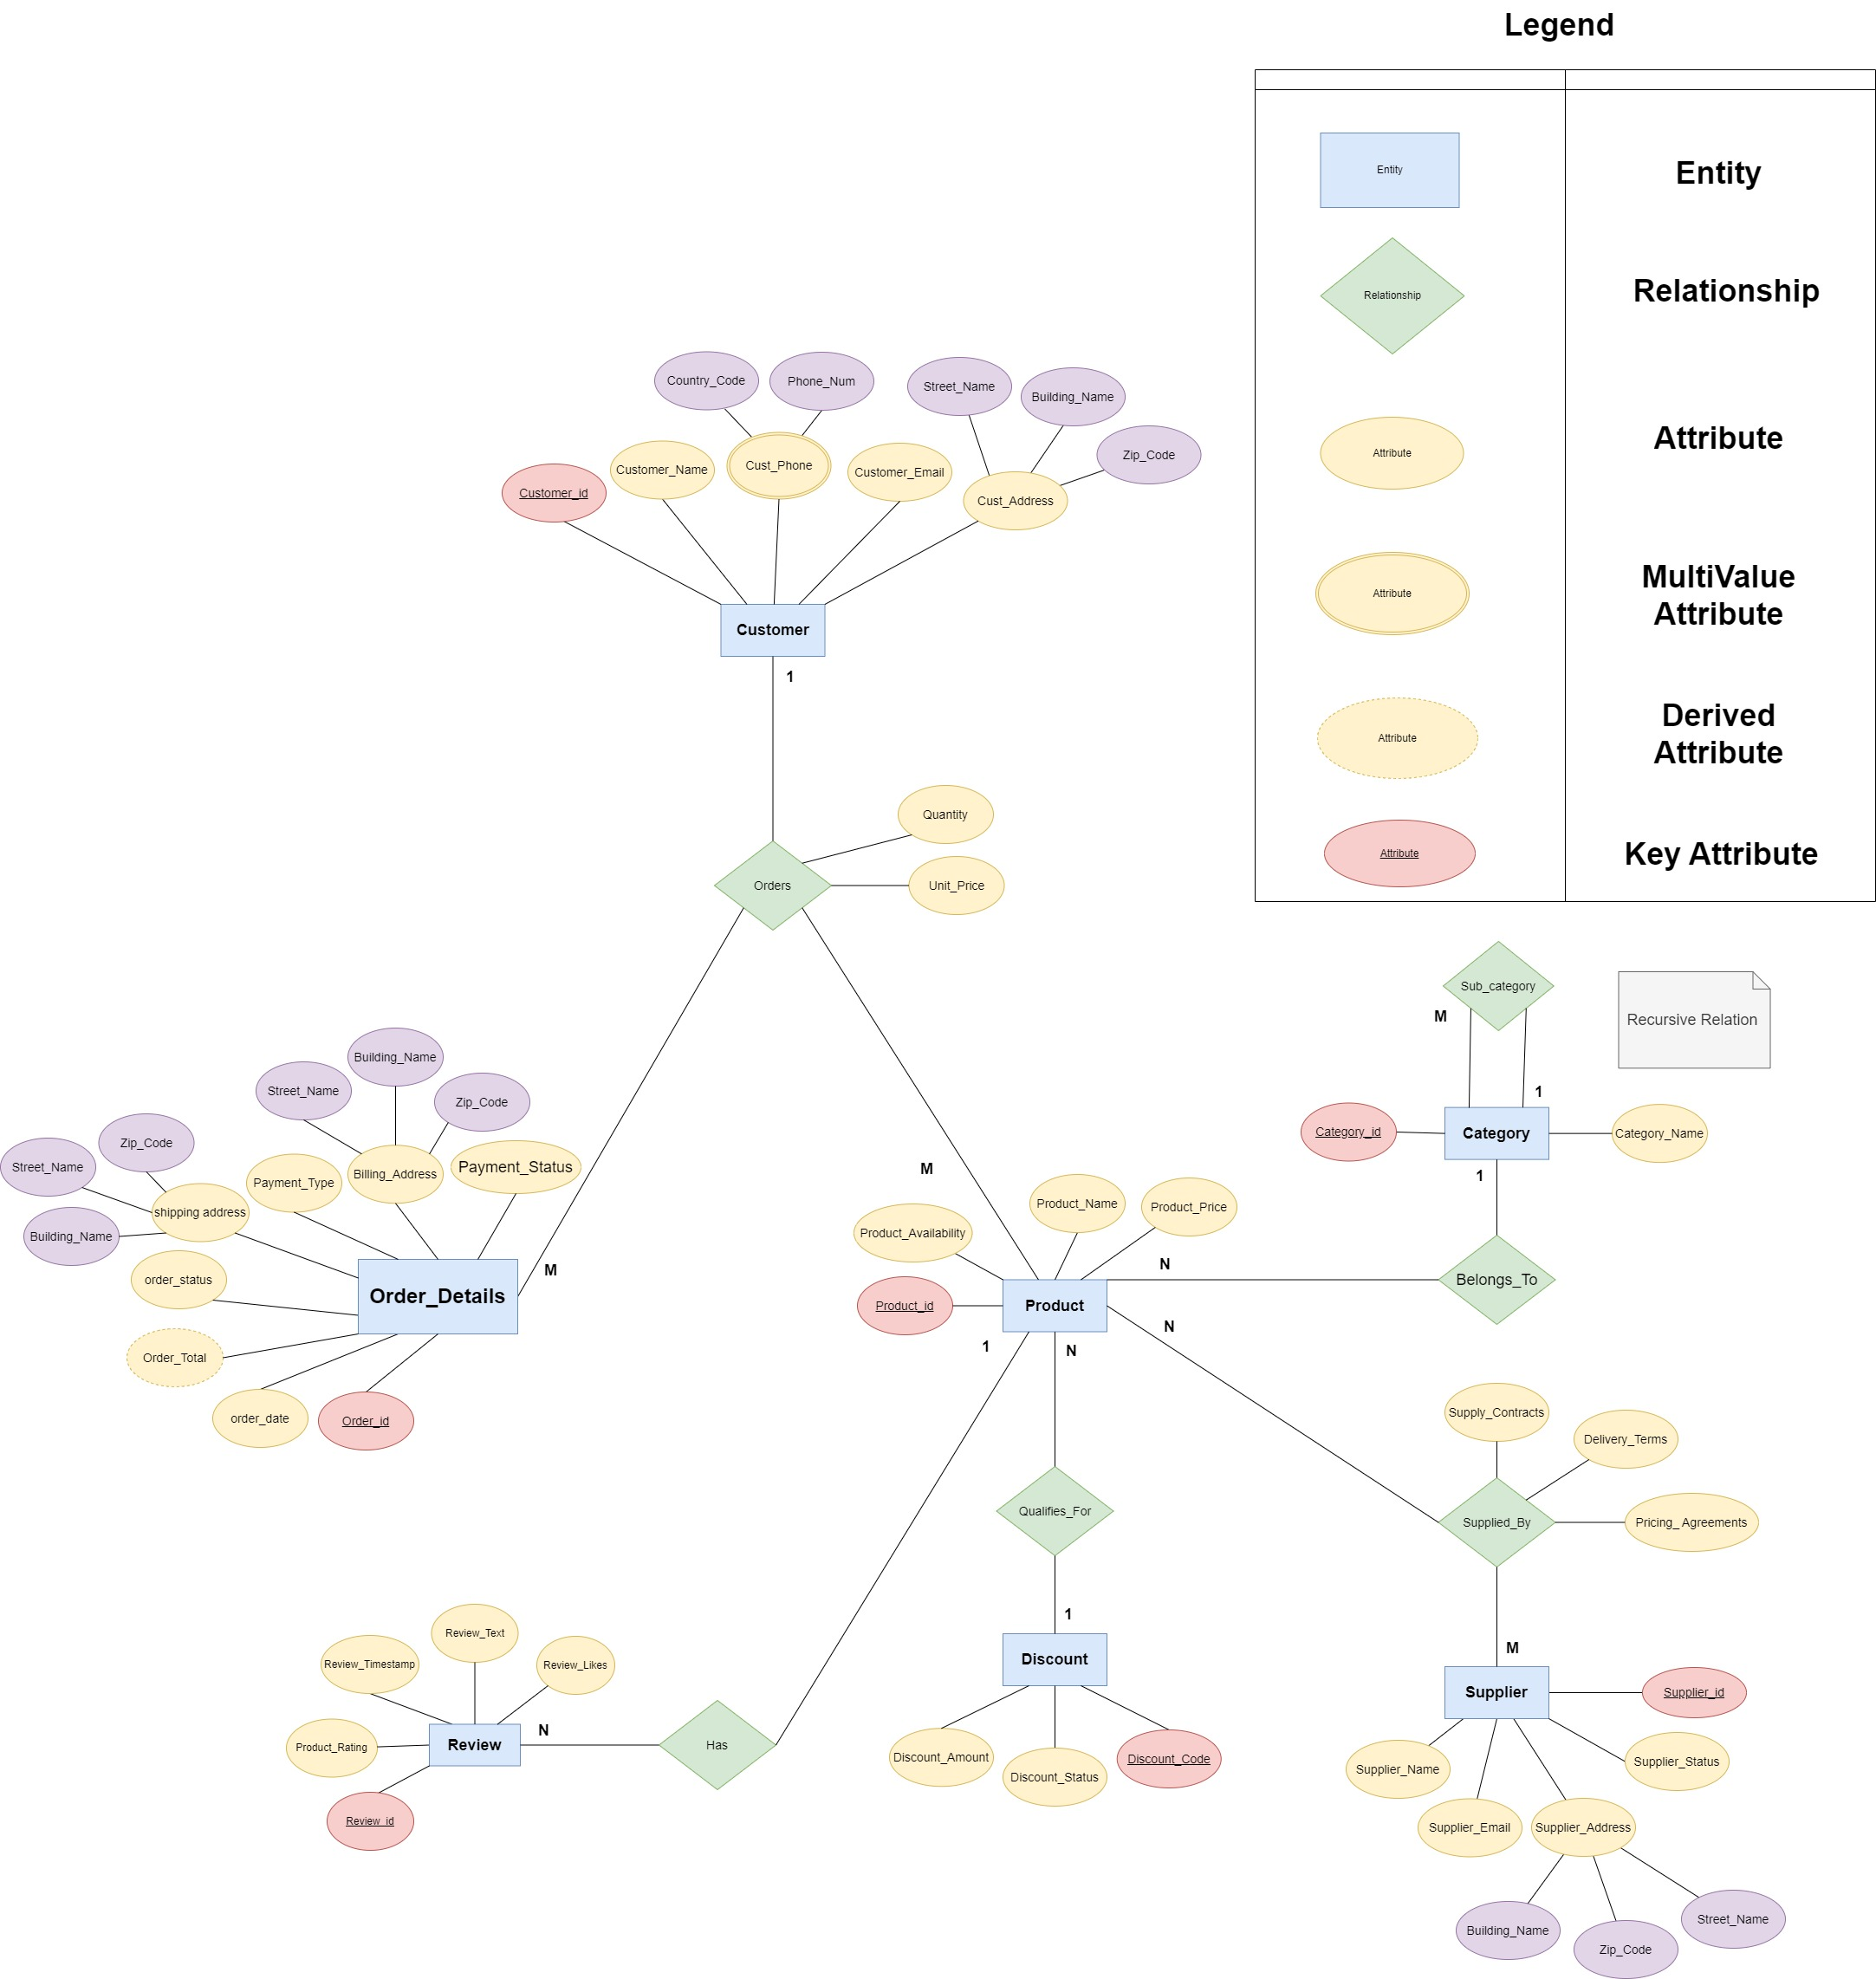
\includegraphics{ERD.jpg}
\caption{ERD}
\end{figure}

The E-R diagram above simulates a real-world e-commerce data ecosystem,
capturing the detailed relationships between entities and attributes
essential for facilitating online transactions. In addition, it provides
a comprehensive view of the e-commerce system, which serves as a
platform for users to browse products, make purchases, and securely
complete their payments.

\hypertarget{assumptions}{%
\subsubsection{1.1.1.Assumptions}\label{assumptions}}

\begin{itemize}
\item
  The company only distributes products within the United Kingdom (UK).
\item
  The Currency used is Pound Sterling (GBP).
\item
  Attributes formats will be aligned with UK standard formats such as
  date , addresses , names \ldots etc
\end{itemize}

\hypertarget{entities-and-attributes}{%
\subsubsection{1.1.2. Entities and
Attributes}\label{entities-and-attributes}}

This section describes and illustrates the entities in the above ERD and
their respective attributes.

\hypertarget{customer}{%
\paragraph{1.1.2.1. Customer}\label{customer}}

Shows us the users who previously have at least once purchased products
and placed an order including information about their names , emails,
and addresses.

\hypertarget{supplier}{%
\paragraph{1.1.2.2. Supplier}\label{supplier}}

Vendors who provide products. Represent the source of the product items.

\hypertarget{product}{%
\paragraph{1.1.2.3 Product}\label{product}}

Describes all products in the stock and available for sale. Provides
information about the model, price, and availability of the products.

\hypertarget{order_details}{%
\paragraph{1.1.2.4 Order\_Details}\label{order_details}}

Emphasises all details related to placed orders including billing,
shipping address, order, payment status, order date, and payment type.

\hypertarget{category-and-sub-category}{%
\paragraph{1.1.2.5 Category and
Sub-Category}\label{category-and-sub-category}}

Category is the broad classification of products that share common
features or are intended for a similar purpose. A sub-category is a more
specific grouping of products within a category based on finer
distinctions or attributes.

Sub-categories fall under a primary category and help to further
organize products into narrower groups, making the product search
process even more straightforward for customers.

\hypertarget{product_discounts}{%
\paragraph{1.1.2.6 Product\_Discounts}\label{product_discounts}}

The voucher number or offer code to be applied to eligible products. The
amount of discount it offers as well as the status of the discount are
the main attributes.

\hypertarget{reviews}{%
\paragraph{1.1.2.7 Reviews}\label{reviews}}

Contains Written comments and rating of product sold by verified buyers,
the likes of the top reviews as well as the time stamp of when the
review was made.

\hypertarget{design-considerations}{%
\section{Design Considerations}\label{design-considerations}}

\hypertarget{absence-of-an-order-entity}{%
\subsection{Absence of an Order
Entity:}\label{absence-of-an-order-entity}}

\begin{itemize}
\item
  The model intentionally skips direct order management. Instead, it
  focuses on product management and customer interactions through
  reviews and payment methods.Additionally, This consideration will
  guarantee that products purchased by customers are not tracked or
  stored by the system to align with privacy policies.
\item
  Order Entity not considered in this ER design in order to follow best
  practices by not having to include orderId as part of product table
  which might affect the overall performance of DB retrieval.
\item
  Customer Engagement: By including Reviews, the model emphasizes
  customer engagement and feedback without directly managing
  transactions.
\item
  Payment Information: Including Payment\_Method without an Order entity
  suggests a pre-registration of payment preferences or a simplified
  wallet storage that could be expanded in the future.
\end{itemize}

\hypertarget{relationship-and-cardinalities}{%
\section{1.1.3. Relationship and
Cardinalities}\label{relationship-and-cardinalities}}

\begin{enumerate}
\def\labelenumi{\arabic{enumi}.}
\tightlist
\item
  Customer Orders Products
\end{enumerate}

A Customer initiates an Order when they purchase products or services.
It is considered for customer management, processing transactions, and
tracking order history. One customer can place multiple orders over
time, each uniquely associated with one customer.

Associative attributes: (Quantity: The number of units of the product
ordered in this line item.), (Unit Price: The price per unit of the
product at the time of the order. This is important as product prices
can vary over time), (Unit\_Sub\_Total : The total cost for this line
item (typically calculated as (Quantity * Unit Price)).

\begin{enumerate}
\def\labelenumi{\arabic{enumi}.}
\setcounter{enumi}{1}
\tightlist
\item
  Customer Has Order Status
\end{enumerate}

This relation will be created when customers order their first product
or service. They will be linked with a particular Order Status
indicating what they ordered, reflecting the current state or
progression throughout the process. One customer can be associated with
multiple order statuses at any given time. Moreover, it is good for
tracking an order's life cycle, allowing for updates, customer
notifications, and management of the order fulfilment process.

\begin{enumerate}
\def\labelenumi{\arabic{enumi}.}
\setcounter{enumi}{2}
\tightlist
\item
  Product Belongs to Category
\end{enumerate}

Each Product is classified under a specific Category where products can
belong to multiple categories e.g., a product that fits into both
``Electronics'' and ``Gadgets''. This enabling customer to browse
products by categories, and helping retailers to manage product listings
more efficiently.

\begin{enumerate}
\def\labelenumi{\arabic{enumi}.}
\setcounter{enumi}{3}
\tightlist
\item
  Category Self-Reference Relation
\end{enumerate}

A category can have multiple subcategories, creating a hierarchically
nested structure and making it easier for users to navigate the product
catalogue. For example, the ``Phones'' category might have ``Apple'' and
``Samsung'' as subcategories, which in turn could have their own
subcategories of different phone models.

\begin{enumerate}
\def\labelenumi{\arabic{enumi}.}
\setcounter{enumi}{4}
\tightlist
\item
  Product Supplied\_By Supplier
\end{enumerate}

The relationship creates a link between the products and their
suppliers. Thereby indicating multiple vendors can supply a product, as
well as supply multiple different products. The relation helps track
inventory sources, manage supplier relationships, and ensure product
availability.

\begin{enumerate}
\def\labelenumi{\arabic{enumi}.}
\setcounter{enumi}{5}
\tightlist
\item
  Product Qualifies\_For Discount
\end{enumerate}

The relation signifying that the product is eligible for certain
promotional discount enabling dynamic pricing strategies, encouraging
sales, and providing customers with various savings opportunities on
different products. In this context and for simplicity the relation
representing one discount code or voucher that is valid to apply on
multiple eligible products.

\begin{enumerate}
\def\labelenumi{\arabic{enumi}.}
\setcounter{enumi}{6}
\tightlist
\item
  Customer Writes a Review
\end{enumerate}

A customer generates or provides reviews that reflect the action of
providing feedback or evaluation for a product or service to improve
product offerings and customer service. One customer can write or submit
multiple reviews for different products or services over time. However,
each review is uniquely associated with one customer.

\hypertarget{logical-schema}{%
\subsection{Logical Schema}\label{logical-schema}}

Customers (\(\underline{Customer_id}\), Customer\_Email, Cust\_F\_Name,
Cust\_L\_Name, Phone\_Country\_Code, Phone\_Num, Cust\_Street\_Name,
Cust\_Building\_Name, Cust\_Zip\_Code)

Products (\(\underline{Product_id}\), \emph{Discount\_Code},
\emph{Category\_id}, Product\_Name, Product\_Price,
Product\_Availability)

Suppliers (\(\underline{Supplier_id}\), Supplier\_Email, Supplier\_Name,
Supplier\_Status, Sup\_Building\_Name, Sup\_Street\_Name,
Sup\_Zip\_Code)

Order\_Details (\(\underline{Order_id}\), \emph{Customer\_id},
Order\_Date, Order\_Total, Order\_Status, S\_Building\_Name,
S\_Street\_Name, S\_Zip\_Code, Street\_Name, B\_Building\_Name,
B\_Street\_Name, B\_Zip\_Code, Payment\_Type, Payment\_Status)

Discounts (\(\underline{Discount_Code}\), Discount\_Status,
Discount\_Amount)

Reviews (\(\underline{Review_id}\), \emph{Product\_id}, Review\_Rating,
Review\_Timestamp, Review\_Text, Review\_Likes)

Categories (\(\underline{Category_id}\), Category\_Name)

SupplierProduct (\(\underline{Supplier_id, Product_id}\),
Supply\_Contracts, Delivery\_Terms, Pricing\_Agreements)

Many to Many relation of Supplier and Product SupplierProduct
(\(\underline{Supplier_id,Product_id}\))

Many to Many relation of Order\_details and Product
ProductOrder\_details (\(\underline{Order_id, Product_id}\), Quantity,
Unit\_Price)

\hypertarget{part-2-data-generation-and-management}{%
\section{Part 2: Data Generation and
Management}\label{part-2-data-generation-and-management}}

\hypertarget{synthetic-data-generation}{%
\subsection{Synthetic Data Generation}\label{synthetic-data-generation}}

After the agreement on the schema mentioned in the previous section, the
team started to generate synthetic data that to some extent, imitated
realistic e-commerce as much as possible.

ChatGPT has been used as the main tool for this step as an alternative
to Mockaroo, as the former produces more structural and logical data
than the latter.

\hypertarget{data-import-and-quality-assurance}{%
\subsection{Data Import and Quality
Assurance}\label{data-import-and-quality-assurance}}

The process was done manually to the very few cells that still don't
make any sense related to e commerce, or it was left blank and AI tools
missed to produce.

\hypertarget{part-3-data-pipeline-generation}{%
\section{Part 3: Data Pipeline
Generation}\label{part-3-data-pipeline-generation}}

\begin{Shaded}
\begin{Highlighting}[]
\CommentTok{\# We need to rename and delete columns like building number, as it does not match or does not exist in the database }
\CommentTok{\# Suppliers amendment }
\NormalTok{Suppliers}\SpecialCharTok{$}\NormalTok{Supplier\_Building\_Number }\OtherTok{\textless{}{-}} \ConstantTok{NULL}
\NormalTok{Suppliers }\OtherTok{\textless{}{-}}\NormalTok{ Suppliers }\SpecialCharTok{\%\textgreater{}\%} \FunctionTok{rename}\NormalTok{(}\AttributeTok{Supplier\_Zip =}\NormalTok{ Supplier\_Zip\_Code)}

\CommentTok{\# Customers amendment }
\NormalTok{Customers }\OtherTok{\textless{}{-}}\NormalTok{ Customers }\SpecialCharTok{\%\textgreater{}\%} \FunctionTok{rename}\NormalTok{(}\AttributeTok{Cust\_Zip =}\NormalTok{ Cust\_Zip\_Code)}
\NormalTok{Customers }\OtherTok{\textless{}{-}}\NormalTok{ Customers }\SpecialCharTok{\%\textgreater{}\%} \FunctionTok{rename}\NormalTok{(}\AttributeTok{Cust\_Country\_Code =}\NormalTok{ Phone\_Country\_Code)}


\CommentTok{\# Order\_details }
\CommentTok{\# Don\textquotesingle{}t have these in the database }
\NormalTok{Order\_details}\SpecialCharTok{$}\NormalTok{Billing\_Building\_Number }\OtherTok{\textless{}{-}} \ConstantTok{NULL}
\NormalTok{Order\_details}\SpecialCharTok{$}\NormalTok{Shipping\_Building\_Number }\OtherTok{\textless{}{-}} \ConstantTok{NULL}

\CommentTok{\#This is one of the ways of doing it , havent do order\_details pending for changes from abigail. }
\NormalTok{RSQLite}\SpecialCharTok{::}\FunctionTok{dbWriteTable}\NormalTok{(con, }\StringTok{"Category"}\NormalTok{, Product\_Category, }\AttributeTok{overwrite=}\ConstantTok{TRUE}\NormalTok{)}
\NormalTok{RSQLite}\SpecialCharTok{::}\FunctionTok{dbWriteTable}\NormalTok{(con, }\StringTok{"Suppliers"}\NormalTok{, Suppliers, }\AttributeTok{overwrite=}\ConstantTok{TRUE}\NormalTok{)}
\NormalTok{RSQLite}\SpecialCharTok{::}\FunctionTok{dbWriteTable}\NormalTok{(con, }\StringTok{"Discounts"}\NormalTok{, Product\_Discounts, }\AttributeTok{overwrite=}\ConstantTok{TRUE}\NormalTok{)}
\NormalTok{RSQLite}\SpecialCharTok{::}\FunctionTok{dbWriteTable}\NormalTok{(con, }\StringTok{"Products"}\NormalTok{, Products, }\AttributeTok{overwrite=}\ConstantTok{TRUE}\NormalTok{)}
\NormalTok{RSQLite}\SpecialCharTok{::}\FunctionTok{dbWriteTable}\NormalTok{(con, }\StringTok{"Customers"}\NormalTok{, Customers, }\AttributeTok{overwrite=}\ConstantTok{TRUE}\NormalTok{)}
\NormalTok{RSQLite}\SpecialCharTok{::}\FunctionTok{dbWriteTable}\NormalTok{(con, }\StringTok{"Reviews"}\NormalTok{, Reviews, }\AttributeTok{overwrite=}\ConstantTok{TRUE}\NormalTok{) }
\NormalTok{RSQLite}\SpecialCharTok{::}\FunctionTok{dbWriteTable}\NormalTok{(con, }\StringTok{"Order\_Items"}\NormalTok{, Order\_Item, }\AttributeTok{overwrite=}\ConstantTok{TRUE}\NormalTok{)}
\NormalTok{RSQLite}\SpecialCharTok{::}\FunctionTok{dbWriteTable}\NormalTok{(con, }\StringTok{"Order\_Details"}\NormalTok{, Order\_details, }\AttributeTok{overwrite=}\ConstantTok{TRUE}\NormalTok{)}
\end{Highlighting}
\end{Shaded}

\hypertarget{count-the-number-of-reviews-for-each-rating-level}{%
\subsubsection{Count the number of reviews for each rating
level}\label{count-the-number-of-reviews-for-each-rating-level}}

\begin{Shaded}
\begin{Highlighting}[]

\KeywordTok{SELECT}\NormalTok{ Product\_Rating, }\FunctionTok{COUNT}\NormalTok{(Product\_Rating) }\KeywordTok{AS}\NormalTok{ Product\_Rating\_Count}
\KeywordTok{FROM}\NormalTok{ Reviews}
\KeywordTok{GROUP} \KeywordTok{BY}\NormalTok{ Product\_Rating;}
\end{Highlighting}
\end{Shaded}

\begin{longtable}[]{@{}lr@{}}
\caption{6 records}\tabularnewline
\toprule\noalign{}
Product\_Rating & Product\_Rating\_Count \\
\midrule\noalign{}
\endfirsthead
\toprule\noalign{}
Product\_Rating & Product\_Rating\_Count \\
\midrule\noalign{}
\endhead
\bottomrule\noalign{}
\endlastfoot
0 & 27 \\
1 & 21 \\
2 & 20 \\
3 & 26 \\
4 & 19 \\
5 & 37 \\
\end{longtable}

\hypertarget{display-all-products-supplied-by-s001-i.e.-apple-in-descending-price}{%
\subsubsection{Display all products supplied by S001 (i.e.~Apple) in
descending
price}\label{display-all-products-supplied-by-s001-i.e.-apple-in-descending-price}}

\begin{Shaded}
\begin{Highlighting}[]

\KeywordTok{SELECT} \OperatorTok{*}
\KeywordTok{FROM}\NormalTok{ Products }
\KeywordTok{WHERE}\NormalTok{ Supplier\_ID }\OperatorTok{=} \OtherTok{"S001"}
\KeywordTok{ORDER} \KeywordTok{BY}\NormalTok{ Product\_Price }\KeywordTok{DESC}\NormalTok{;}
\end{Highlighting}
\end{Shaded}

\begin{longtable}[]{@{}
  >{\raggedright\arraybackslash}p{(\columnwidth - 12\tabcolsep) * \real{0.1028}}
  >{\raggedright\arraybackslash}p{(\columnwidth - 12\tabcolsep) * \real{0.2150}}
  >{\raggedleft\arraybackslash}p{(\columnwidth - 12\tabcolsep) * \real{0.1308}}
  >{\raggedright\arraybackslash}p{(\columnwidth - 12\tabcolsep) * \real{0.1963}}
  >{\raggedright\arraybackslash}p{(\columnwidth - 12\tabcolsep) * \real{0.1121}}
  >{\raggedright\arraybackslash}p{(\columnwidth - 12\tabcolsep) * \real{0.1121}}
  >{\raggedright\arraybackslash}p{(\columnwidth - 12\tabcolsep) * \real{0.1308}}@{}}
\caption{9 records}\tabularnewline
\toprule\noalign{}
\begin{minipage}[b]{\linewidth}\raggedright
Product\_ID
\end{minipage} & \begin{minipage}[b]{\linewidth}\raggedright
Product\_Name
\end{minipage} & \begin{minipage}[b]{\linewidth}\raggedleft
Product\_Price
\end{minipage} & \begin{minipage}[b]{\linewidth}\raggedright
Product\_Availability
\end{minipage} & \begin{minipage}[b]{\linewidth}\raggedright
Category\_ID
\end{minipage} & \begin{minipage}[b]{\linewidth}\raggedright
Supplier\_ID
\end{minipage} & \begin{minipage}[b]{\linewidth}\raggedright
Discount\_Code
\end{minipage} \\
\midrule\noalign{}
\endfirsthead
\toprule\noalign{}
\begin{minipage}[b]{\linewidth}\raggedright
Product\_ID
\end{minipage} & \begin{minipage}[b]{\linewidth}\raggedright
Product\_Name
\end{minipage} & \begin{minipage}[b]{\linewidth}\raggedleft
Product\_Price
\end{minipage} & \begin{minipage}[b]{\linewidth}\raggedright
Product\_Availability
\end{minipage} & \begin{minipage}[b]{\linewidth}\raggedright
Category\_ID
\end{minipage} & \begin{minipage}[b]{\linewidth}\raggedright
Supplier\_ID
\end{minipage} & \begin{minipage}[b]{\linewidth}\raggedright
Discount\_Code
\end{minipage} \\
\midrule\noalign{}
\endhead
\bottomrule\noalign{}
\endlastfoot
P1857653 & Apple MacBook Model 22 & 1885.11 & Limited Availability &
CAT2 & S001 & NA \\
P5084276 & Apple Watch Model 133 & 1813.57 & Limited Availability & CAT9
& S001 & DISCOUNT11 \\
P8699814 & Apple iPhone Model 50 & 1679.01 & In Stock & CAT3 & S001 &
DISCOUNT16 \\
P0038292 & Apple MacBook Model 23 & 1464.99 & In Stock & CAT2 & S001 &
NA \\
P4637031 & Apple iPhone Model 49 & 1421.52 & Out of Stock & CAT3 & S001
& NA \\
P4081539 & Apple MacBook Model 24 & 1239.98 & In Stock & CAT2 & S001 &
NA \\
P1961681 & Apple Watch Model 135 & 1184.14 & Limited Availability & CAT9
& S001 & NA \\
P8038804 & Apple Watch Model 134 & 619.29 & Limited Availability & CAT9
& S001 & NA \\
P6530444 & Apple iPhone Model 51 & 63.14 & Limited Availability & CAT3 &
S001 & NA \\
\end{longtable}

\hypertarget{head}{%
\section{\textless\textless\textless\textless\textless\textless\textless{}
HEAD}\label{head}}

\hypertarget{top-5-orders-with-the-highest-total-value-after-discount}{%
\subsubsection{Top 5 Orders with the highest total value after
discount}\label{top-5-orders-with-the-highest-total-value-after-discount}}

\begin{Shaded}
\begin{Highlighting}[]

\KeywordTok{SELECT}\NormalTok{ a.Order\_ID, a.Quantity, a.Sum\_Price, b.Discount\_Amount, }\FunctionTok{ROUND}\NormalTok{(a.Quantity }\OperatorTok{*}\NormalTok{ a.Sum\_Price }\OperatorTok{{-}}\NormalTok{ b.Discount\_Amount) }\KeywordTok{AS}\NormalTok{ Total\_Value}
\KeywordTok{FROM}\NormalTok{ Order\_Items a, Discounts b}
\KeywordTok{WHERE}\NormalTok{ a.Product\_ID }\OperatorTok{=}\NormalTok{ b.Product\_ID}
\KeywordTok{ORDER} \KeywordTok{BY}\NormalTok{ Total\_Value }\KeywordTok{DESC}
\KeywordTok{LIMIT} \DecValTok{5}\NormalTok{;}
\end{Highlighting}
\end{Shaded}

\begin{longtable}[]{@{}lrrrr@{}}
\caption{5 records}\tabularnewline
\toprule\noalign{}
Order\_ID & Quantity & Sum\_Price & Discount\_Amount & Total\_Value \\
\midrule\noalign{}
\endfirsthead
\toprule\noalign{}
Order\_ID & Quantity & Sum\_Price & Discount\_Amount & Total\_Value \\
\midrule\noalign{}
\endhead
\bottomrule\noalign{}
\endlastfoot
O5667066 & 24 & 39942.96 & 42.99 & 958588 \\
O5667071 & 23 & 38486.36 & 6.75 & 885180 \\
O5667053 & 21 & 33319.86 & 8.50 & 699709 \\
O8148246 & 20 & 33823.00 & 85.25 & 676375 \\
O5667082 & 19 & 24974.74 & 23.50 & 474497 \\
\end{longtable}

\begin{quote}
\begin{quote}
\begin{quote}
\begin{quote}
\begin{quote}
\begin{quote}
\begin{quote}
96fcad5708fdb65f1064084b247f679829ce7186
\end{quote}
\end{quote}
\end{quote}
\end{quote}
\end{quote}
\end{quote}
\end{quote}

\begin{Shaded}
\begin{Highlighting}[]
\CommentTok{\# I want to create a for loop so we can do it one shot. Still trying to think through it. }
\end{Highlighting}
\end{Shaded}


\end{document}
